\documentclass[10pt,twoside]{article}
\usepackage[T1]{fontenc}
\usepackage{harvard}
\usepackage{url}
\usepackage{graphicx}
\graphicspath{ {../images/} }
\pagestyle{plain}

\def\all{all}
\ifx\files\all \typeout{Including all files.} \else %\typeout{Including only \files.} \includeonly{\files} \fi

% Keywords command
\providecommand{\keywords}[1]
{
  \small	
  \textbf{\textit{Keywords---}} #1
}

\title{eSports Branding: A Preliminary Literature Review}
\author{Pieter Joubert \\
	Vega School Bordeaux \\
	}

\date{\today}
% Hint: \title{what ever}, \author{who care} and \date{when ever} could stand 
% before or after the \begin{document} command 
% BUT the \maketitle command MUST come AFTER the \begin{document} command! 
\begin{document}

\maketitle
\keywords{Digital Sponsorship, Brand Leadership, Game Design, Game Development, Structured Literature Review.}

\section{Subject Area}
Brand Leadership and Management
\section{Introduction}

The field of digital sponsorship, specifically in the field of eSports, is one that requires further investigation, according to various authors \cite{huettermann2020esports}, \cite{Elasri-Ejjaberi2020}. Furthermore it is unclear to what extent game design and level design effect how gamers perceive brand placement in digital games \cite{hwang2017effects}.

This paper will thus explore the current state of the literature regarding Branding in eSports, and more specifically the link between Game and Level Design and Brand Placement in eSports.

The Research Question that this paper wishes to explore is: To what extent has the link between Game and Level Design and Brand Placement in eSports been explored in the literature?

\section{Literature}
The field of Digital Sponsorship is still nascent, but there is a growing body of literature exploring various aspects of Digital Sponsorship. Some authors are comparing Digital Sponsorship to traditional forms of Sports Sponsorship \cite{huettermann2020esports}, others are exploring the possibility of Brand Harm and Digital Sponsorship \cite{Freitas2019} and finally authors are generally commenting on the lack of detailed research within this field and performing their own exploratory literature reviews \cite{Elasri-Ejjaberi2020}.

To help underpin the study Aaker's Brand Identity model will be used to provide theoretical structure and classification to the literature reviewed and the summary of the literature that will be produced. \cite{aaker2012brand}

\section{Methodology}

The research data, being academic literature can be classified as highly mediated, but unstructured, using the mixed methods framework of Plowright \cite{plowright2011using}. This classification naturally leads to performing a Structured Literature Review \cite{petticrew2008systematic}.

To ensure that the literature that is reviewed is structured into a logical format, Aaker's Brand Identity model will be used. This review will focus primarily on the issue of Brand Identity, so the four brand identity perspectives (brand as a product, an organization, a person, and a symbol) will be used as the primary categories for classification \cite{aaker2012brand}. Each of these primary categories will then be sub-divided into the appropriate sub-category as shown below:

\begin{figure}[h]
\caption{Brand Identity Model Adapted from Aaker}
\centering
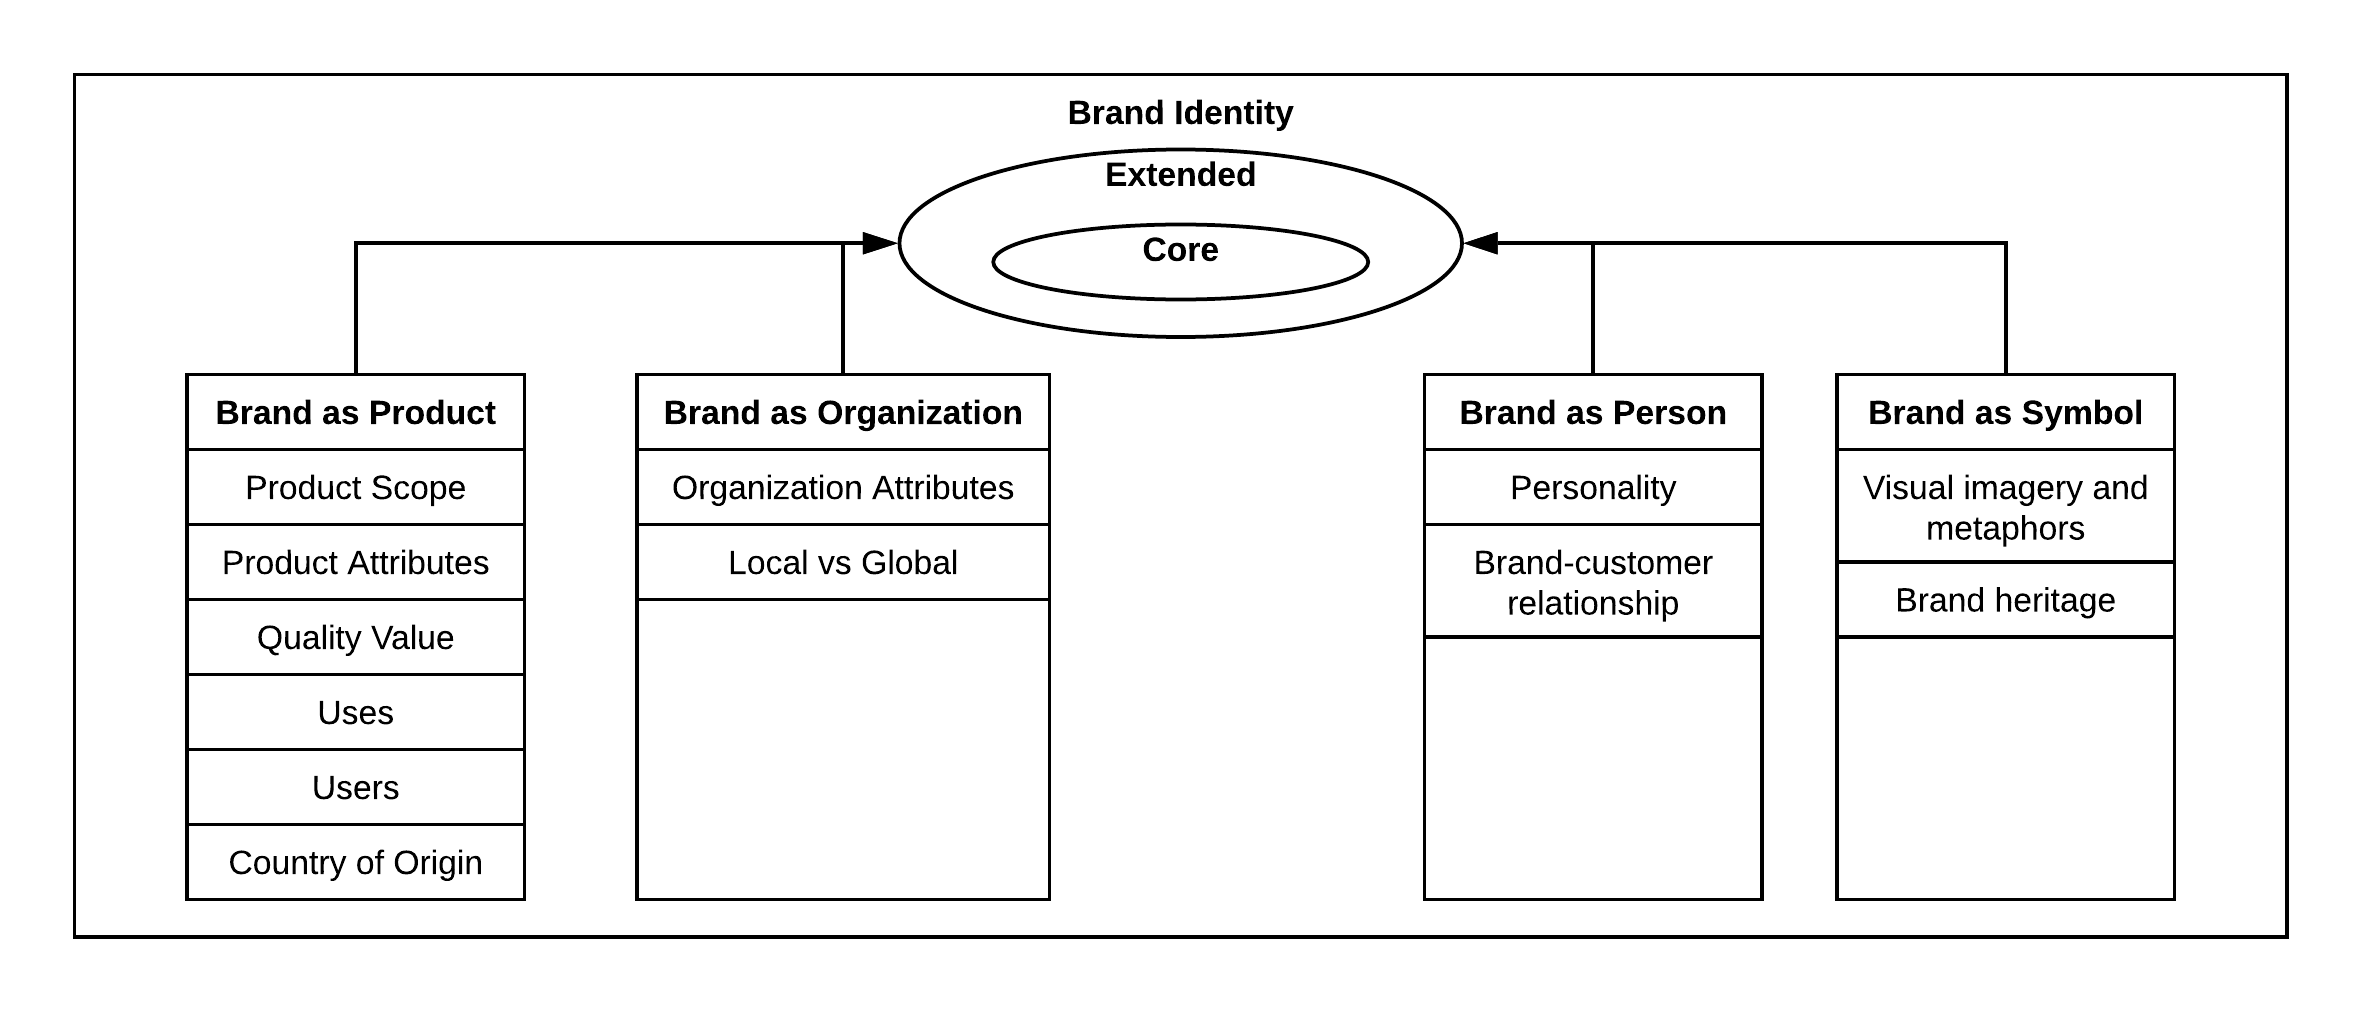
\includegraphics[width=1\textwidth]{BrandIdentityModel.png}
\end{figure}

This approach will link the sources reviewed to the theoretical framework of Aaker's Brand Identity model, and through doing so, identify any gaps in the literature.

This approach will also identify any aspects of the literature that are not present within Aaker's model, and provide scope for adapting the Brand Identity model.

Any additional themes of interest will also be noted as a means to further explore various other aspects of the eSports Branding space.

The following process was followed to perform this preliminary:
\subsection{Process}

An inital investigation of the literature was done with the following parameters:
\begin{enumerate}
	\item Search term: \emph{esports branding}
	\item Date range: Since 2020
\end{enumerate}

This was used to identify overarching themes as well as high quality sources that could be used for further indepth examination.

Finally the themes will be tabulated, summarised and discussed, especially to identify any existing gaps in the literature. The themes will also be linked to Aakers Brand Identity model.

\section{Data Analysis}

\subsection{Preliminary identification of sources and themes}

In this preliminary phase, using the search term: \emph{esports branding} and the data range: Since 2020: eight sources were analysed in detail. It was decided to stop after these sources as (a) this was only a preliminary investigation, (b) high quality sources had been identified, and (c), theme saturation had been reached at this point.

It is interesting to note at this point that because the field of esports branding is so novel, there is limited literature regarding the concept and a lot of the literature tends to cross-reference each other. A number of the resources were also student dissertations and/or theses, which provided helpful overviews of the literature.

These were the top 10 themes identified from the sources.

\begin{center}
	\begin{tabular}{|l|c|}
		\hline	
		Theme & Frequency \\
		\hline
		content & 9 \\
		influencers & 9 \\
		livestream & 8 \\
		social media & 7 \\
		sponsorship & 6 \\
		player brand & 5 \\
		as Person & 5 \\
		engagement & 5 \\
		authenticity & 4 \\
		demographics & 4 \\
		non-endemic & 4 \\
		branding & 4 \\
		ROI & 3 \\
		\hline
	\end{tabular}
\end{center}

From these results (please note that a single theme could occur multiple times within a source), it is clear that the most important aspects are all related to the content produced by players, via livestreaming and social media, that enhance themselves, their teams and their sponsors as a brand. This content must be engaging and authentic.

The only aspect of Aaker's Brand model that appears in this top 10 is "the Brand as a Person", and the relationship the consumer has with the Brand. This aspect gets a little muddled as this deals both with the sponsor's brand, the game's brand and the player/teams' brand(s).

Two other interesting themes snuck into the top 10, namely the issues of endemic vs. non-endemic brands and the question of ROI for sponsors of eSports.

Finally, many of the sources detailed extensively the demographics of eSports consumers, which is useful for providing a convincing argument as to the value of using eSports as a marketing avenue for a Brand.

\subsection{Link to Brand Identity Model}

Devlving deeper into the themes that were identified and the links to Aakers Brand model results in the following diagram:

\begin{figure}[h]
\caption{Brand Identity Model Adapted from Aaker}
\centering
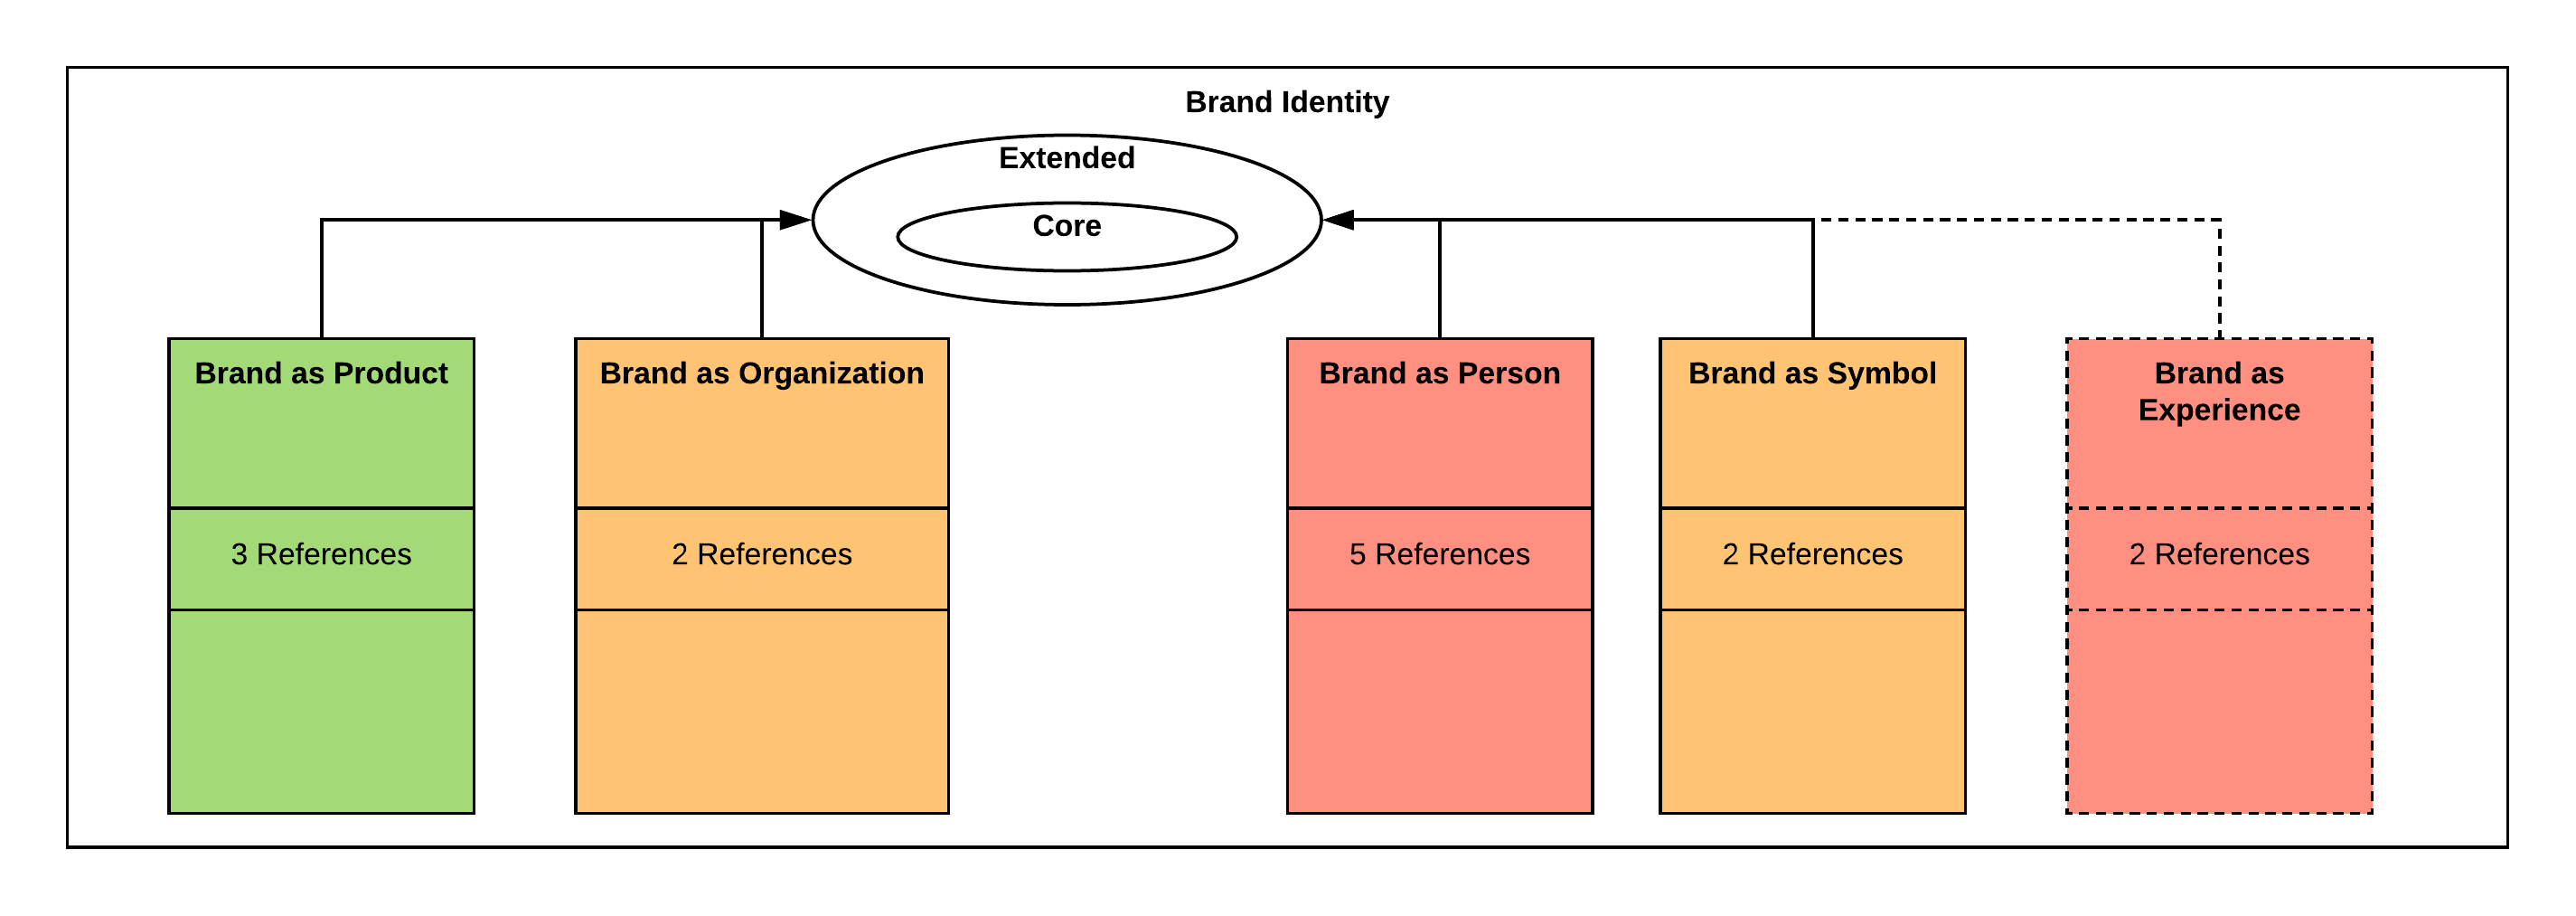
\includegraphics[width=1\textwidth]{BrandIdentityModelUpdated.png}
\end{figure}

Most importantly is that the Brand as a Person aspect of Brand Identity was the most commonly referred to, secondly was Brand as a Product and finally Brand as an Organization and Symbol had the fewest occurrences.

Many sources referred to the experience of the Brand, or to the Brand as an Experience. This additional section is included in the figure as a possible extension of Aaker's model.

\section{Ethical Clearance}
No participants of any kind will be included in the study so no ethical clearance will be required.

\section{Findings and Results}


\section{Limitations of the Study}
The study will be time limited to explore the most recent literature in the field, and will be limited to eSports games only, to ensure that the study is focused.

\bibliographystyle{myharvard}
\bibliography{../esports_slr, ../PHD_literature}

\end{document}
